% Dit werk is gelicenseerd onder de licentie Creative Commons Naamsvermelding-GelijkDelen 4.0 Internationaal. Ga naar http://creativecommons.org/licenses/by-sa/4.0/ om een kopie van de licentie te kunnen lezen.
\chapter{Gelijkvormigheid}
\label{sec:Gelijkvormigheid}

%%%%%%%%%%%%%%%%%%%%%%%%%%%%%%%%%%%%%%%%%%%%%%%%%%%%%%%%%%%%%%%%%%%%%%%%%%%%%%%%%%%%%%%%%%%%
	\section{Inleiding}
	\label{sec:Gelijkvormigheid Inleiding}
In het vorige hoofdstuk hebben we de differentiaalvergelijkingen die de stroming beheersen afgeleid. Voor praktische problemen is een oplossing voor deze vergelijkingen vinden alles behalve eenvoudig. Er moet gebruik gemaakt worden van numerieke oplossingsmethoden en zelfs dan is de modellering van turbulentie moeilijk.

Vaak is het nodig om experimentele resultaten te bekomen. Experimenten met prototypes zijn echter vaak niet mogelijk omwille van de kosten van deze prototypes of de schaal van het prototype. Het is bijvoorbeeld niet mogelijk een nieuwe vorm van romp voor een olietanker tijdens de ontwerpfase op volle schaal te testen om de stromingsweerstand te bepalen. Om deze redenen wordt vaak gebruik gemaakt van experimenten op schaalmodellen.

In dit hoofdstuk zullen we de gebruiksvoorwaarden voor schaalmodellen opstellen en een methode ontwikkelen om experimenteel bepaalde gegevens te vertalen naar de volle schaal geometrie. Het werkelijke probleem zal vanaf nu het prototype genoemd worden, terwijl het schaalmodel waarop experimenten gebeuren het model genoemd wordt. Grootheden die betrekking hebben op het model worden met een accent genoteerd.

%%%%%%%%%%%%%%%%%%%%%%%%%%%%%%%%%%%%%%%%%%%%%%%%%%%%%%%%%%%%%%%%%%%%%%%%%%%%%%%%%%%%%%%%%%%%
	\section{Voorwaarden voor gelijkvormigheid}
	\label{sec:Voorwaarden voor gelijkvormigheid}
		\subsection{Geometrische gelijkvormigheid}
De eerste en meest logische voorwaarde voor gelijkvormigheid is geometrische gelijkvormigheid. Deze stelt dat alle lengte verhoudingen gelijk moeten zijn voor het model en het prototype. In Figuur \ref{fig:geometrische gelijkvormigheid} betekent dit dat de verhouding van koorde tot dikte in het model gelijk moet zijn aan de verhouding van koorde tot dikte in het prototype.
\begin{equation}
	\dfrac{T'}{C'} = \dfrac{T}{C}
	\label{eqn:geometrische gelijkvormigheid vleugel}
\end{equation}
Of meer algemeen:
\begin{equation}
	\dfrac{\Delta \vt{x}_i'}{\Delta \vt{x}_j'} = \dfrac{\Delta \vt{x}_i}{\Delta \vt{x}_j} \quad, \forall i,j
	\label{eqn:geometrische gelijkvormigheid}
\end{equation}
\begin{figure}[htb]
	\centering
	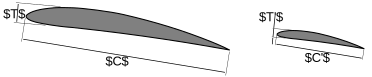
\includegraphics{fig/gelijkvormigheid/Geometrische_gelijkvormigheid}
	\caption{Geometrische gelijkvormigheid}
	\label{fig:geometrische gelijkvormigheid}
\end{figure}
Deze gelijkheid van lengteverhoudingen moet kloppen voor alle verhoudingen. Zo zal bijvoorbeeld ook de ruwheid van de oppervlakken mee geschaald moeten worden. Dit kan in de praktijk gebeuren door andere materialen of bewerkingen te kiezen. Sommige geometrische details zullen de interessante grootheden slechts weinig beïnvloeden. Het weglaten van zulke details is dan ook zeer interessant om de kosten van het model te drukken. De kunst bestaat erin de details die weinig invloed zullen hebben te herkennen.
	\subsection{Kinematische gelijkvormigheid}
Als tweede voorwaarde beschouwen we kinematische gelijkvormigheid. Dit komt er op neer dat het snelheidsveld voor het model en prototype gelijkvormig zijn. De verhoudingen tussen eender welke snelheden in het model moet dus gelijk zijn aan de verhouding van snelheden op de corresponderende punten in het prototype:
\begin{equation}
	\dfrac{\left. \vt{v}' \right|_{x_i',y_i'}}{\left. \vt{v}' \right|_{x_j',y_j'}} = \dfrac{\left. \vt{v} \right|_{x_i,y_i}}{\left. \vt{v} \right|_{x_j,y_j}} \quad, \forall i,j
	\label{eqn:kinematische gelijkvormigheid}
\end{equation}
Voor de meeste problemen zijn bovenstaande voorwaarden echter niet voldoende.
	\subsection{Dynamische gelijkvormigheid}
De laatste voorwaarde voor gelijkvormigheid is dynamische gelijkvormigheid. Dit wil zeggen dat elke verhouding van krachten in het model gelijk moet zijn aan de corresponderende verhouding in het prototype.
\begin{equation}
	\dfrac{\left. \vt{F}'_a \right|_{x_i',y_i'}}{\left. \vt{F}'_b \right|_{x_j',y_j'}} = \dfrac{\left. \vt{F}_a \right|_{x_i,y_i}}{\left. \vt{F}_b \right|_{x_j,y_j}} \quad, \forall a,b,i,j
	\label{eqn:dynamische gelijkvormigheid}
\end{equation}
Vaak wordt de traagheidskracht die aangrijpt op een fluïdumdeeltje als referentiekracht genomen:
\begin{equation}
	\dfrac{\left. \vt{F}' \right|_{x',y'}}{\left. \vt{F}'_{\mathrm{traagheid}} \right|_{x',y'}} = \dfrac{\left. \vt{F} \right|_{x,y}}{\left. \vt{F}_{\mathrm{traagheid}} \right|_{x,y}}
	\label{eqn:dynamische gelijkvormigheid traagheid}
\end{equation}
Om deze voorwaarde te garanderen kunnen we een hulpmiddel gebruiken: het dimensieloos maken van de toepasbare vergelijkingen.

%%%%%%%%%%%%%%%%%%%%%%%%%%%%%%%%%%%%%%%%%%%%%%%%%%%%%%%%%%%%%%%%%%%%%%%%%%%%%%%%%%%%%%%%%%%%
	\section{Dimensieloze getallen}
Beschouwen we de bewegingsvergelijking van een deeltje in een niet samendrukbare stroming met viskeuze krachten (\ref{eqn:navier-stokes vergelijkingen}) en projecteren we deze op de stoomrichting:
\begin{equation}
	\rho \frac{\partial v}{\partial t} + \rho v \frac{\partial v}{\partial s} = -\frac{\partial p}{\partial s} + \rho g_s + \mu \frac{\partial^2 v}{\partial s^2}
	\label{eqn:navier-stokes geprojecteerd}
\end{equation}
Elke term in deze vergelijking heeft de eenheid kracht per volume (\unit{N/m^3}). De verschillende termen stellen de verschillende krachten voor die op een fluïdumdeeltje uitgeoefend worden. De term $-\frac{\diff p}{\diff s}$ is afkomstig van de kracht ten gevolge van drukverschillen per eenheid van volume. De term $\rho g_s$ is afkomstig van de zwaartekracht per eenheid van volume geprojecteerd in de $s$ richting. De term $\mu \frac{\partial^2 v}{\partial s^2}$ stelt de viskeuze kracht voor inwerkend op het deeltje. De term $\rho \frac{\partial v}{\partial t}$ stelt de lokale versnelling van het deeltje voor en de term $\rho v \frac{\diff v}{\diff s}$ stelt de convectieve versnelling van een deeltje voor en kunnen we dus voorstellen als de traagheidskracht per eenheid van volume.

We kunnen de veranderlijken in deze vergelijking allen schrijven als een dimensieloze veranderlijke vermenigvuldigd met een vaste referentie. Kiezen we bijvoorbeeld $D_{\text{ref}}$ als referentie voor de lengte, $t_{\text{ref}}$ als referentie voor de tijd  $v_{\text{ref}}$ als referentie voor de snelheid en $p_{\text{ref}}$ als referentie voor de druk. De dimensieloze veranderlijken noteren we met een $^*$: 
\begin{align}
	s &= s^* D_{\text{ref}} \nonumber \\
	v &= v^* v_{\text{ref}}  \\
	t &= t^* t_{\text{ref}} \nonumber \\
	p &= p^* p_{\text{ref}} \nonumber
	\label{eqn:referentie grootheden}
\end{align}
Indien we deze waarden invullen in (\ref{eqn:navier-stokes geprojecteerd}) verkrijgen we:
\begin{equation}
	\rho \frac{\partial v^* v_{\text{ref}}}{\partial t^* t_{\text{ref}}} + \rho v^* v_{\text{ref}} \frac{\partial v^* v_{\text{ref}}}{\partial s^* D_{\text{ref}}} = -\frac{\partial p^* p_{\text{ref}}}{\partial s^*D_{\text{ref}}} + \rho g_s + \mu \frac{\partial^2 v^* v_{\text{ref}}}{\partial s^{*2} D_{\text{ref}}^2}
\end{equation}
Merk nu echter op dat dat de referentie tijd niet onafhankelijk is. Willen we een consistente dimensieloze snelheid bekomen dan moet $t_{\text{ref}} = D_{\text{ref}}/v_{\text{ref}}$:
\begin{equation}
	\frac{\rho v_{\text{ref}}^2}{D_{\text{ref}}} \frac{\partial v^*}{\partial t^*} + \frac{\rho v_{\text{ref}}^2}{D_{\text{ref}}}v^* \frac{\partial v^*}{\partial s^*} = -\frac{p_{\text{ref}}}{D_{\text{ref}}} \frac{\partial p^*}{\partial s^*} + \rho g_s + \frac{\mu v_{\text{ref}}}{D_{\text{ref}}^2} \frac{\partial^2 v^*}{\partial s^{*2}}
	\label{eqn:navier-stokes dimensieloos}
\end{equation}
Elke term in de vergelijking is nu geschreven als een constante maal een dimensieloze veranderlijke. Elke van de constante factoren moet dus een referentie waarde voor een bepaalde kracht voorstellen zoals hierboven besproken. We kunnen de verhoudingen van de krachten die inwerken op een deeltje dus schrijven als het quotiënt van de factoren in vergelijking (\ref{eqn:navier-stokes dimensieloos}). De voorwaarde voor dynamische gelijkvormigheid (\ref{eqn:dynamische gelijkvormigheid traagheid}) kunnen we nu bekomen door de quotiënten van de factoren in (\ref{eqn:navier-stokes dimensieloos}) constant te houden voor model en prototype.

Delen we (\ref{eqn:navier-stokes dimensieloos}) door $\frac{\rho v_{\text{ref}}^2}{D_{\text{ref}}}$ (de referentiefactor voor traagheidskracht) verkrijgen we:
\begin{equation}
	\frac{\partial v^*}{\partial t^*} + v^* \frac{\partial v^*}{\partial s^*} =- \frac{p_{\text{ref}}}{\rho v_{\text{ref}}^2} \frac{\partial p^*}{\partial s^*} + \frac{g_s D_{\text{ref}}}{v_{\text{ref}}^2} + \frac{\mu}{\rho v_{\text{ref}} D_{\text{ref}}} \frac{\partial^2 v^*}{\partial s^{*2}}
	\label{eqn:navier-stokes dimensieloos traagheid}
\end{equation}
In de eerste term van (\ref{eqn:navier-stokes dimensieloos traagheid}) zien we de dimensieloze deeltjesversnelling terug. De overige termen stellen de verhoudingen van krachten voor die op het deeltje inwerken. Indien we deze constant kunnen houden tussen model en prototype, wordt de beweging van een deeltje in het model en het prototype beschreven door dezelfde differentiaalvergelijking. De relatieve beweging van elk deeltje zal dan ook hetzelfde zijn. We hebben dus een voorwaarde die dynamische gelijkvormigheid garandeert.

De coëfficiënten in (\ref{eqn:navier-stokes dimensieloos traagheid}) kunnen allen gerelateerd worden aan dimensieloze getallen. Zo kan vergelijking (\ref{eqn:navier-stokes dimensieloos traagheid}) geschreven worden als:
\begin{equation}
	\frac{\partial v^*}{\partial t^*} + v^* \frac{\partial v^*}{\partial s^*} =  -\text{Eu} \frac{\partial p^*}{\partial s^*} + \frac{1}{\text{Fr}^2} + \frac{1}{\text{Re}} \frac{\partial^2 v^*}{\partial s^{*2}}
	\label{eqn:navier-stokes dimensieloze getallen}
\end{equation}
De voorkomende dimensieloze getallen zijn het Euler getal, het Froude getal en het Reynolds getal. Deze relateren respectievelijk de druk kracht, zwaartekracht en viskeuze kracht tot de traagheidskracht. In de definitie van de dimensieloze getallen wordt het subscript ''ref'' ook weggelaten aangezien het hier steeds over de referentiegrootheden gaat. Enkele in de stromingsmechanica vaak voorkomende dimensieloze getallen zijn:
\begin{align}
	\mathrm{Re} &= \dfrac{\rho v D}{\mu} &= \dfrac{v D}{\nu} = \dfrac{\mathrm{traagheidskracht}}{\mathrm{viskeuze krachten}} \label{eqn:Reynolds} \\
	\mathrm{Eu} &= \dfrac{p}{\rho v^2}   &= \dfrac{\mathrm{drukkracht}}{\mathrm{traagheidskracht}} \label{eqn:Euler} \\
	\mathrm{Fr} &= \dfrac{v}{\sqrt{g D}} &= \sqrt{\dfrac{\mathrm{traagheidskracht}}{\mathrm{zwaartekracht}}} \\
	\mathrm{Ma} &= \dfrac{v}{c}          &= \dfrac{\mathrm{traagheidskracht}}{\mathrm{samendrukbaarheidskrachten}}
	\label{eqn:Dimensieloze getallen}
\end{align}
Een zeer belangrijke en zeer vaak gebruikte grootheid in de fluïdum mechanica is het Reynoldsgetal, genoemd naar Osbourne Reynolds. Dit getal vormt de verhouding van de traagheidskracht tot de viskeuze krachten die inwerken op een fluïdum deeltje. Wanneer het Reynoldsgetal voor een bepaalde stroming zeer laag is zullen viskeuze krachten de stroming overheersen. Zo'n stroming wordt ook kruipende stroming (E: creeping flow) genoemd. Wanneer het Reynoldsgetal echter zeer groot is zullen viskeuze krachten weinig invloed hebben. In dit geval kunnen we gebruik maken van de vergelijkingen van Euler en Bernoulli die in het vorige hoofdstuk afgeleid werden. Bij hoge Reynoldsgetallen zal er echter een ander fenomeen optreden: turbulentie. We zullen dieper op dit fenomeen ingaan in hoofdstuk \ref{sec:Uitwendige stroming} en hoofdstuk \ref{sec:Inwendige stroming}.

Het Froude getal, genoemd naar William Froude, geeft de verhouding tussen de traagheidskrachten en de zwaartekracht weer. In de meeste stromingen zal de zwaartekracht enkel zorgen voor een lineaire drukverdeling met de hoogte in de vloeistof. Bij een specifieke klasse stromingsproblemen heeft de zwaartekracht echter wel een belangrijke invloed op de beweging van individuele deeltjes. Dit zijn problemen waarbij er een vrij vloeistof oppervlak aanwezig is (E: Free surface flow). Voorbeelden zijn de stroming van een rivier onder invloed van de zwaartekracht, golven in de oceaan ten gevolge van de wind of de boeggolf van een schip dat zich door het water beweegt.

%%%%%%%%%%%%%%%%%%%%%%%%%%%%%%%%%%%%%%%%%%%%%%%%%%%%%%%%%%%%%%%%%%%%%%%%%%%%%%%%%%%%%%%%%%%%
	\section{Buckingham-Pi theorema}
Een andere kijk op dimensieloze grootheden kunnen we bekomen door middel van dimensie analyse. Elke vergelijking met een fysische betekenis moet namelijk homogeen in de eenheden zijn. Dit wil zeggen dat alle termen in de vergelijking dezelfde eenheden moeten hebben. Als eenvoudig voorbeeld kunnen we de tweede wet van Newton $F=ma$ aanhalen. Hierin heeft het linkerlid de eenheid van kracht [\unit{N}]. Het rechterlid heeft als eenheid [\unit{kg \frac{m}{s^2}}] wat in het meter-kilogram-seconde stelsel net de definitie van de eenheid van kracht [\unit{N}] is. Een meer fluïdummechanish voorbeeld is de vergelijking van Bernoulli (\ref{eqn:vergelijking van Bernoulli}). Hierin hebben alle termen de eenheid [\unit{\frac{J}{m^3}}] ofwel energie per eenheid van volume. Elke fysische vergelijking (en dus elke vergelijking in deze cursus) moet op deze manier homogeen zijn in de eenheden.

Elke fysiche grootheid heeft een eenheid die op een bepaalde manier gerelateerd kan worden aan enkel basiseenheden. Enkele veel voorkomende grootheden zijn gegeven in Tabel \ref{tab:grootheden}. Hierin is te zien dat de dimensies allen gevormd kunnen worden met behulp van enkele basis dimensies: L als dimensie van lengte, M als dimensie van massa , T als dimensie van tijd, en $\theta$ als dimensie van temperatuur. We kunnen elke fysische vergelijking dus ook schrijven met behulp van deze basis dimensies. Zo heeft de vergelijking van Bernoulli de dimensie ML$^{-1}$T$^{-2}$.
\begin{table}[htb]
	\centering
	\begin{tabular}{lll}
		\hline
		Grootheid                   & Dimensie   & Eenheid \\
		\hline
		Lengte                       & \unit{L}                      &   \unit{m} \\
		Massa                        & \unit{M}                      &   \unit{kg} \\
		Tijd                         & \unit{T}                      &   \unit{s} \\
		Dichtheid                    & \unit{ML^{-3}}                &   \unit{kg/m^3} \\
		Druk                         & \unit{ML^{-1}T^{-2}}          &   \unit{N/m^2} \\	
		Dynamische viscositeit       & \unit{MT^{-1}L^{-1}}          &   \unit{Pa s} \\
		Energie (arbeid)             & \unit{ML^{2}T^{-2}}           &   \unit{J} \\
		Impuls                       & \unit{MLT^{-1}}               &   \unit{kg m/s} \\
		Kinematische viscositeit     & \unit{L^{2}T^{-1}}            &   \unit{m^2/s} \\
		Kracht                       & \unit{MLT^{-2}}               &   \unit{N} \\
		Snelheid                     & \unit{LT^{-1}}                &   \unit{m/s} \\
		Vermogen                     & \unit{ML^{2}T^{-3}}           &   \unit{J/s} \\
		Versnelling                  & \unit{LT^{-2}}                &   \unit{m/s^2} \\
		Volume                       & \unit{L^3}                    &   \unit{m^3} \\
		Temperatuur                  & \unit{\theta}                 &   \unit{K} \\
		Conductiecoëfficiënt         & \unit{MT^{-3} \theta^{-1}}    &   \unit{W/m^2 K} \\	
		Energie (warmte)             & \unit{MLT^{-2}}               &   \unit{J} \\
		Warmteoverdrachtscoëfficiënt & \unit{MT^{-3}L\theta^{-1}}    &   \unit{W/m K} \\
		\hline
	\end{tabular}
	\caption{Vaak voorkomende grootheden met hun dimensie en eenheden}
	\label{tab:grootheden}
\end{table}

Het Buckingham-pi theorema stelt dat wanneer een fysische grootheid $a$ afhankelijk is van $n$ parameters $a_1$ tot $a_n$ waarvan $k$ grootheden onafhankelijke dimensies hebben:
\begin{equation}
	a = f(a_1,a_2,...,a_n)
\end{equation}
Dan kan deze uitdrukking herschreven worden tot een dimensieloze vergelijking met slechts $n-k$ dimensieloze parameters:
\begin{equation}
	\pi = \phi(\pi_1,\pi_2,...,\pi_{n-k})
\end{equation}
Edgar Buckingham formaliseerde dit principe in 1914 en presenteerde een manier om de dimensieloze parameters op een gestructureerde manier te vinden. Het principe werd echter reeds gebruikt door Baron Rayleigh in 1877. Het theorema kan formeel bewezen worden, dit valt echter buiten het bereik van deze cursus. Geïnteresseerde lezers worden verwezen naar \cite{Yarin2012} waar het thema zeer uitgebreid beschouwd wordt.

\begin{voorbeeld}
	Om de kracht van het theorema aan te tonen beschouwen we bij wijze van voorbeeld de stroming van water rond een scheepsschroef. We zijn geïnteresseerd in de kracht die de schroef uitoefent op de stroming en hebben hier een aantal experimenten voor uitgevoerd. Uit de experimenten blijkt dat de kracht afhankelijk is van de snelheid van de stroming, de dichtheid, de viscositeit, het toerental van de schroef en de diameter van de schroef:
	\begin{equation*}
		F = f(v,\rho,\nu,N,D)
		\label{eqn:dimensieanalyse, voorbeeld}
	\end{equation*}
	De dimensies in deze relatie zijn: $v$: LT$^{-1}$, $\rho$: ML$^{-3}$, $\nu$: L$^{2}$T$^{-1}$, $N$: T$^{-1}$, $D$: L.
	
	Hierin zijn slechts 3 grootheden dimensioneel onafhankelijk. Zo kan bijvoorbeeld de dimensie van $N$ geschreven worden als LT$^{-1}$/L, de dimensie van $v$ gedeeld door die van $D$ en de dimensie van $\nu$ kunnen we bekomen als de dimensie van $D$ maal de dimensie van $v$.  In termen van het Buckingham-pi theorema is $n=5$ en $k=3$. We zullen de relatie dus herschrijven als een dimensieloze vergelijking met $n-k=2$ parameters:
	\begin{equation}
		\pi = \phi(\pi_1,\pi_2)
	\end{equation}
	Door even naar de betrokken parameters te kijken en uit de voorgaande analyse kunnen we de $\pi$ termen gemakkelijk terug vinden. Deze worden:
	\begin{align*}
		\pi &= \frac{F}{\rho v^2 D^2} \\
		\pi_1 &= \frac{v D}{\nu} \\
		\pi_2 &= \frac{N D}{v}
	\end{align*}
	De dimensieloze relatie wordt dus:
	\begin{equation*}
		\frac{F}{\rho v^2 D^2} = \phi(\frac{v D}{\nu},\frac{N D}{v})
	\end{equation*}
	De $\pi$ termen in deze relatie zijn nu ook heel herkenbaar. In het linkerlid vinden we een dimensieloze kracht. De functie in het rechterlid heeft twee parameters. De eerste herkennen we als het Reynoldsgetal. De tweede is het dimensieloze toerental van de schroef, of de verhouding tussen de tipsnelheid en de stroomsnelheid (de snellopendheid).
	
	We kunnen de relatie die oorspronkelijk 5 parameters had dus schrijven als een relatie met slechts 2 parameters. Deze relatie kunnen we (indien de experimenten echt gebeurd zijn) eenvoudig weergeven in een grafiek door een set met krommen weer te geven. Bijvoorbeeld de dimensieloze kracht in functie van het Reynoldsgetal voor verschillende waarden van het dimensieloze toerental. Met behulp van deze grafiek kunnen we de kracht voor elke schroef die geometrisch gelijkvormig is, in elk fluïdum met elke snelheid en elk toerental berekenen.
	\begin{center}
		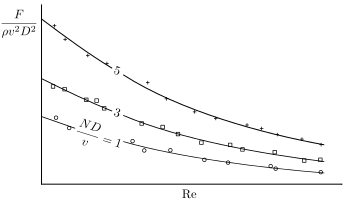
\includegraphics{fig/gelijkvormigheid/dimensieanalysevoorbeeld}
	\end{center}	
	Indien de analyse op voorhand gebeurd is kan zelfs het aantal nodige experimenten sterk beperkt worden, van bijvoorbeeld $2^5=32$ experimenten, om een lineair verband te bepalen tot $2^2=4$ experimenten. Hiervoor is wel een goede inschatting van de invloedrijke parameters nodig.

\end{voorbeeld}